A concepção da ideia do projeto foi desenvolver uma aplicação completa para gestão de vendas, focando na geração do pedido e entrega, sendo essa para qualquer ramo de atividade. Porém, notou-se a falta de exploração de serviços em outro nicho de mercado ainda não explorado e sem concorrentes, com foco somente na otimização da entrega, em que não é preciso disputar clientes com grandes empresas maduras no assunto.
 
A aplicação desenvolvida foca no gerenciamento das rotas de entregas dos pedidos gerados via sistemas de vendas já operantes, necessitando apenas da disponibilização de uma API no formato de arquivo JSON (\autoref{fig:drHttpAPI}), essa compondo-se de dados essenciais para realização da integração automática abordada na próxima Seção.
 
  \begin{figure}[H]
    \centering
    \caption{Delivery Routes - Requisição HTTP}
    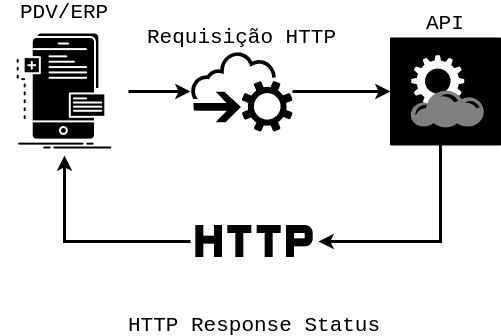
\includegraphics[width=0.6\textwidth]{./dados/figuras/fig16}
    \fonte{\citeonline{iFood}}
    \label{fig:drHttpAPI}
\end{figure}

Primeiramente, é preciso entender os possíveis status e o fluxo de um pedido integrado na Delivery Routes, ambos representados na \autoref{tab:drStatusPedido} e na \autoref{fig:drStatusPedido}.

\begin{table}[H]
    \centering
    \caption{Delivery Routes - Status do pedido
    \label{tab:drStatusPedido}}
\begin{tabular}{|l|l|}
\hline
\textbf{Status} & \textbf{Descrição} \\ \hline
PLACED & Indica que um pedido pode ser integrado no sistema. \\ \hline
CONFIRMED & Indica um pedido disponível para entrega. \\ \hline
INTEGRATED & Indica um pedido vinculado à uma entrega. \\ \hline
CANCELLED & Indica um pedido que foi cancelado. \\ \hline
DISPATCHED & Indica um pedido que foi despachado ao cliente. \\ \hline
DELIVERED & Indica um pedido que foi entregue pelo motoboy. \\ \hline
CONCLUDED & Indica um pedido que foi concluído pelo administrador. \\ \hline
\end{tabular}
    \fonte{Adaptada de \citeonline{iFood}}
\end{table}
 
\begin{figure}[H]
    \centering
    \caption{Delivery Routes - Fluxo do status do pedido}
    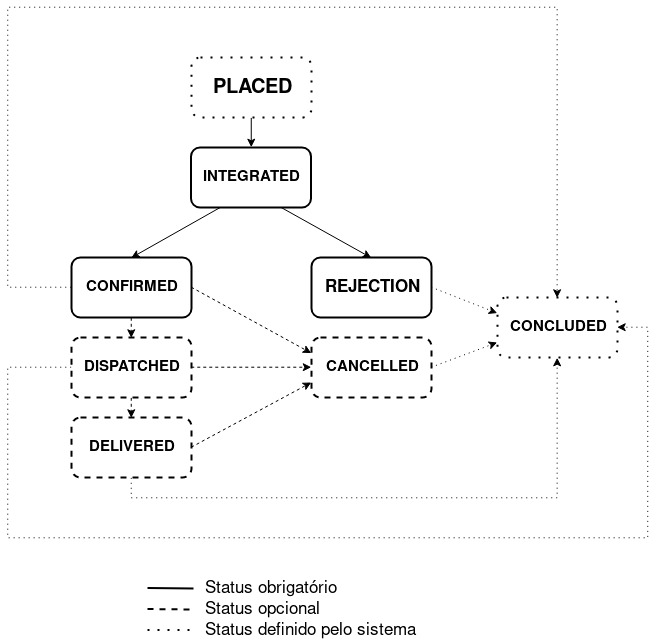
\includegraphics[width=0.6\textwidth]{./dados/figuras/fig15}
    \fonte{\citeonline{iFood}}
    \label{fig:drStatusPedido}
\end{figure}

%%%Se o valor da coluna token_access é diferente ao hash da sessão siginfica que o usuário fez um novo login e gerou um novo hash. Neste caso podemos deslogar o usuário, caso os valores não se coinsidam.

Na \autoref{fig:drLogin} é possível visualizar o acesso ao módulo de gerenciamento, com autenticação apenas para administradores, realizada via e-mail e senha, cujo cadastro é efetuado por meio do link \textit{Register a new membership}. Habilitando a opção \textit{Remember Me}, o controle de única sessão por usuário é ativado, por intermédio de um \textit{hash} gerado no momento do login. É disponibilizado também o link \textit{I forgot my password} para realizar a recuperação da senha, mediante a confirmação de um e-mail existente na base de dados.

\begin{figure}[H]
    \centering
    \caption{Delivery Routes - Login}
    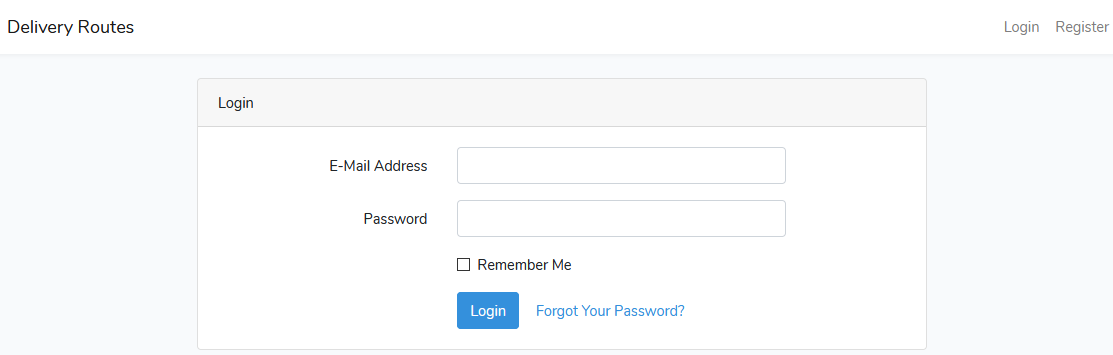
\includegraphics[width=0.4\textwidth]{./dados/figuras/fig7}
    \fonte{Autor}
    \label{fig:drLogin}
\end{figure}

%https://laravel.com/docs/5.7/hashing
O Laravel, juntamente com o Eloquent ORM, disponibiliza a implementação de autenticação de maneira muito simples, por meio do comando \textit{php artisan make:auth}, onde, com poucas instruções e linhas de código, é possível montar a estrutura de cadastro de usuário, recuperação de senha e memória de sessão de maneira extremamente segura, devido ao algoritmo \textit{Bcrypt}
\footnote{Método de criptografia do tipo \textit{hash} adaptativo para senhas que apresenta uma segurança maior em relação à maioria dos outros métodos criptográficos por meio da implementação da variável “custo”, que é proporcional à quantidade de processamento necessária para criptografar a senha \cite{bcrypt}.}
, utilizado para realizar a criptografia da senha.
%%% Conhecido como \textit{hash} adaptativo, pois pode permanecer resistente à ataques do tipo “força-bruta” com o tempo usando custos maiores de processamento

Ao realizar login, o usuário é redirecionado à \textit{dashboard} do sistema, uma interface gráfica que fornece visualização fácil e rápida dos principais indicadores de desempenho, atualizados em tempo real, obtendo assim valores e médias relevantes sobre o processo de negócios. 

Destaca-se na \autoref{fig:drDashboard}, além de indicadores de: Pedidos em aberto, Pedidos em rota, Motoboys disponíveis e Pedidos concluídos, uma barra de menus contendo: Cadastros (Motoboys e Pagamentos) e Movimentos (Entregas e Pedidos Em Aberto).

\begin{figure}[H]
    \centering
    \caption{Delivery Routes - Dashboard}
    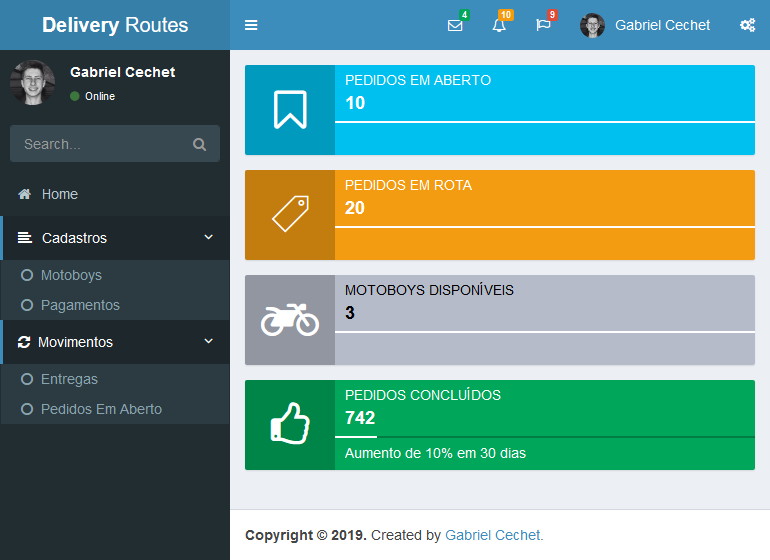
\includegraphics[width=1.0\textwidth]{./dados/figuras/fig13}
    \fonte{Autor}
    \label{fig:drDashboard}
\end{figure}

\newpage
%http://repositorio.ufu.br/handle/123456789/22185
Este projeto foi desenvolvido em duas frentes: um desenvolvimento \textit{front-end} e outro \textit{back-end}. O \textit{front-end} foi baseado em um modelo, ou \textit{template}, chamado Pratt, uma implementação em Blade do tema AdminLTE 5.4 (desenvolvido com Bootstrap). Já o \textit{back-end} foi feito utilizando o \textit{framework} Laravel, na linguagem PHP, como comentado anteriormente.

O Bootstrap, é a biblioteca de componentes \textit{front-end} mais popular do mundo \cite{bootstrap}, e é voltado principalmente para o desenvolvimento de projetos mobile. Todos os componentes oferecidos, como alertas, cartões e formulários, são responsivos, ou seja, eles se redimensionam, se escondem, diminuem ou ficam maiores dependendo do tamanho do dispositivo em que a página é renderizada. Atualmente a biblioteca está na versão 4, o que trouxe muitas melhorias em relação a versão 3, como a simplificação dos componentes de navegação. No entanto, a versão usada pelo AdminLTE ainda é a 3.0 e por isso esta é a versão utilizada neste projeto.

O AdminLTE é um \textit{template} para desenvolvimento de \textit{dashboards} ou painéis de controle. Possui código-aberto, construído usando Bootstrap 3 e design responsivo. Por ser de código-aberto, dúvidas ou problemas encontrados podem ser postados no repositório do projeto no GitHub
\footnote{https://github.com/acacha/adminlte-laravel}, onde qualquer membro da comunidade pode prestar ajuda e propor soluções.

O Pratt é uma implementação baseada no \textit{template} responsivo AdminLTE, que por sua vez utiliza o \textit{framework} Bootstrap. Utilizar projetos como o Pratt como base para desenvolver outras aplicações reduz o tempo necessário para iniciar o desenvolvimento e ajuda a evitar possíveis problemas de configurações que um programador pode encontrar. 

Dessa forma, o Pratt vem com uma configuração pronta do Webpack (\autoref{fig:webpack}), um \textit{module blunder}, cujo principal objetivo, além de automatizar processos como a ofuscação, minificação e outras operações de pré-processamento de código, é permitir que o código seja escrito de forma modular, o que faz com que o desenvolvedor possa aproveitar todas as vantagens provindas do uso do \textit{module blunder}, sem ter que se preocupar com sua configuração inicial.

\begin{figure}[H]
    \centering
    \caption{Webpack - Module blunder}
    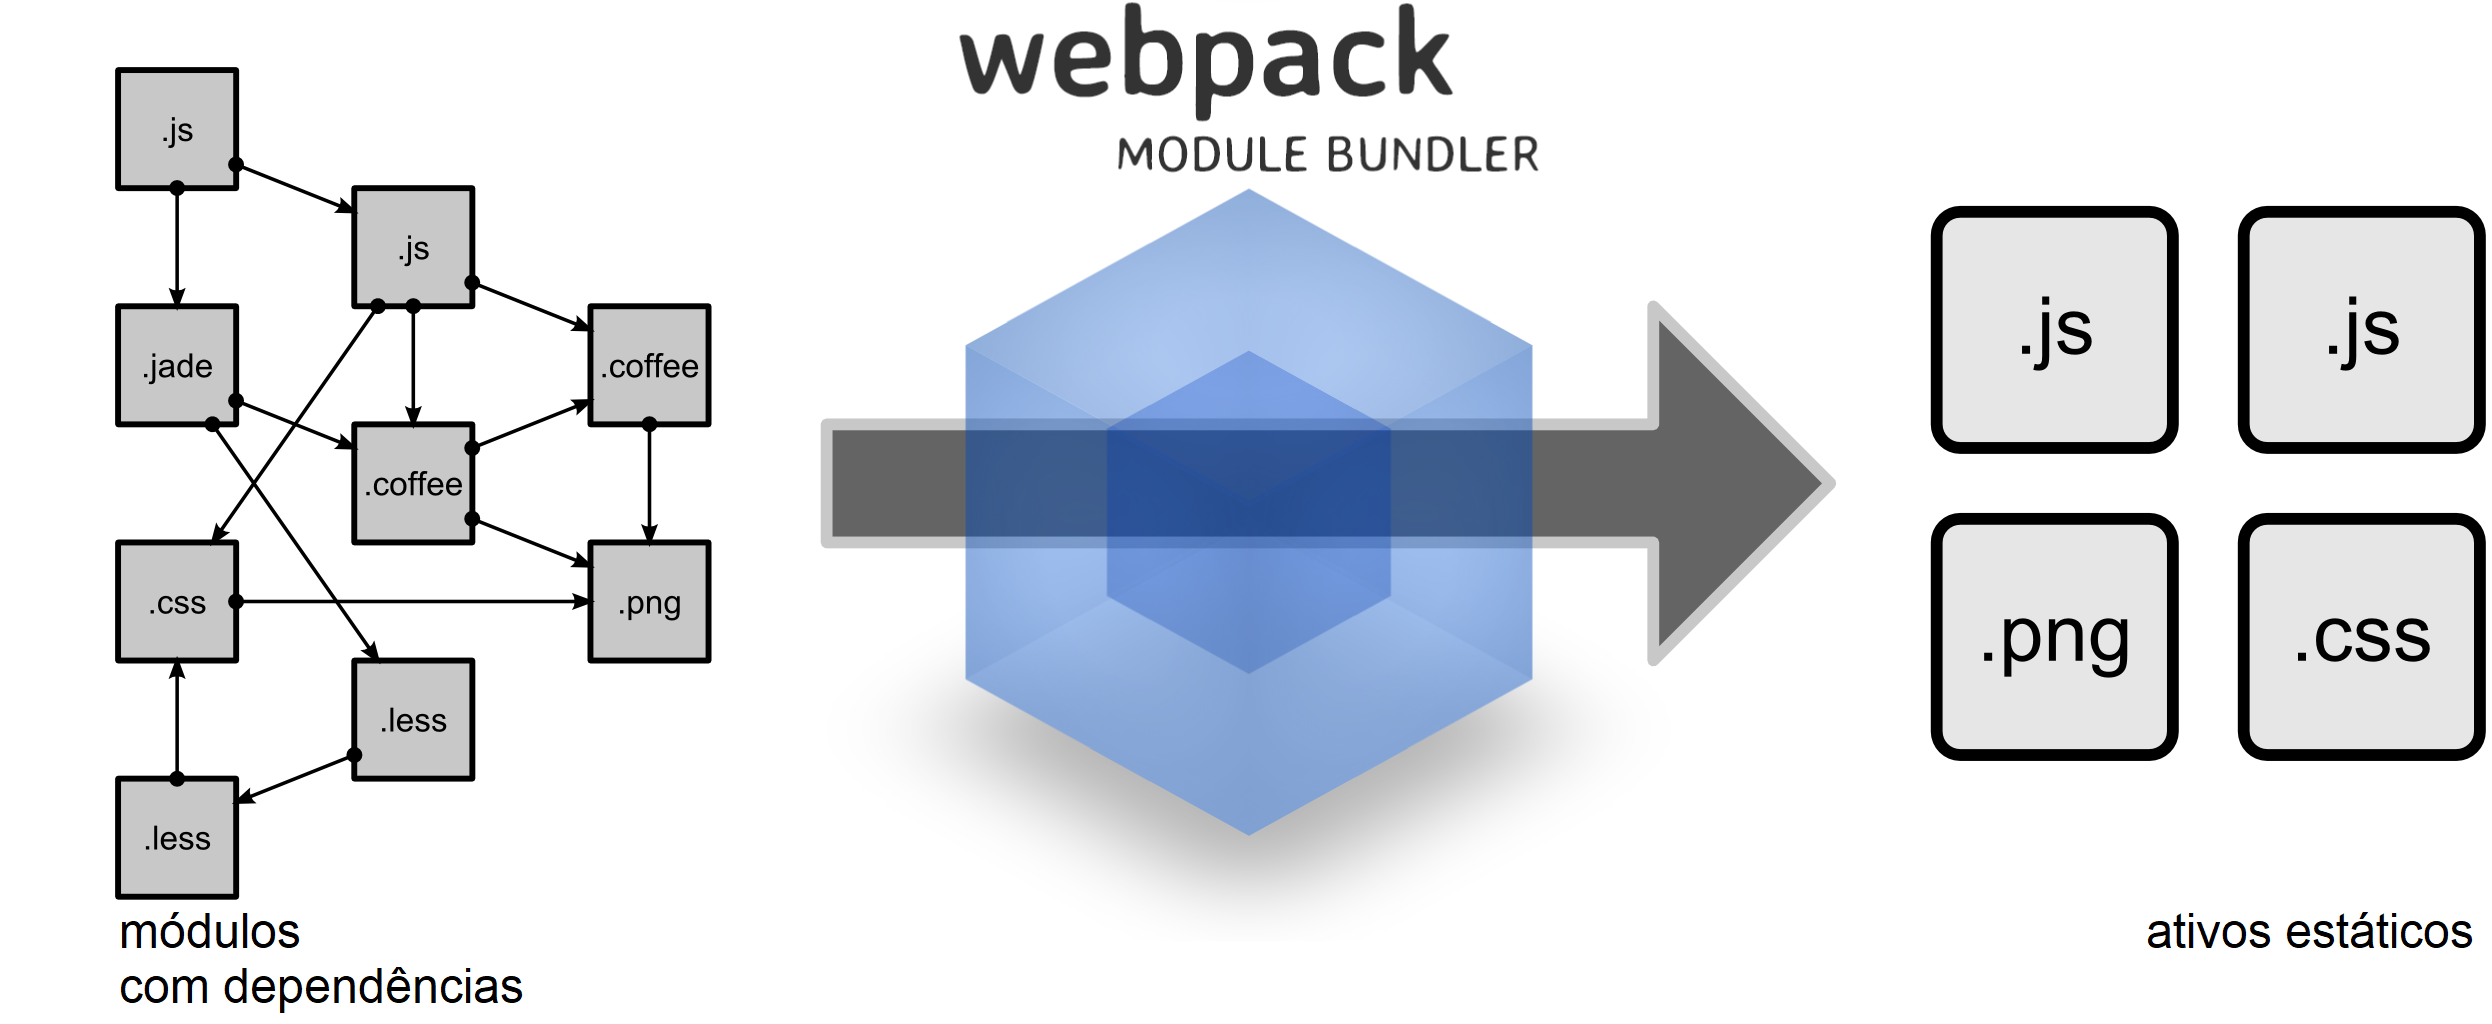
\includegraphics[width=0.8\textwidth]{./dados/figuras/fig17}
    \fonte{Adaptada de \citeonline{webpack}}
    \label{fig:webpack}
\end{figure}

\newpage
Ao selecionar a opção de menu “Motoboys”, o usuário consegue, então, gerenciá-los. Conforme é mostrado na \autoref{fig:drListaMotobys}, há uma listagem com o identificador, nome, CPF, e-mail, telefone e data de criação dos registros cadastrados na base de dados. A listagem também conta com botões para editar, excluir ou criar um registro. A edição do registro é apresentada na \autoref{fig:drEdicaoMotoby}.

\begin{figure}[H]
    \centering
    \caption{Delivery Routes - Lista de motoboys}
    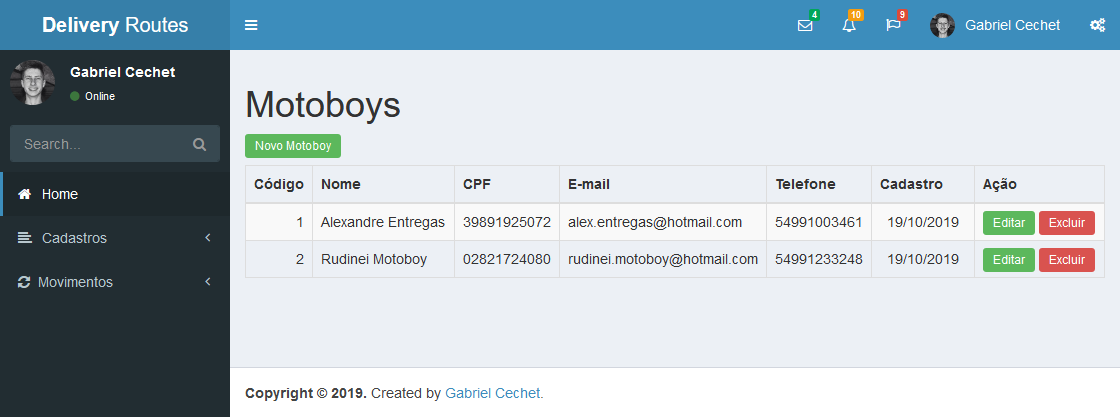
\includegraphics[width=1.0\textwidth]{./dados/figuras/fig18}
    \fonte{Autor}
    \label{fig:drListaMotobys}
\end{figure}

\begin{figure}[H]
    \centering
    \caption{Delivery Routes - Edição do motoboy}
    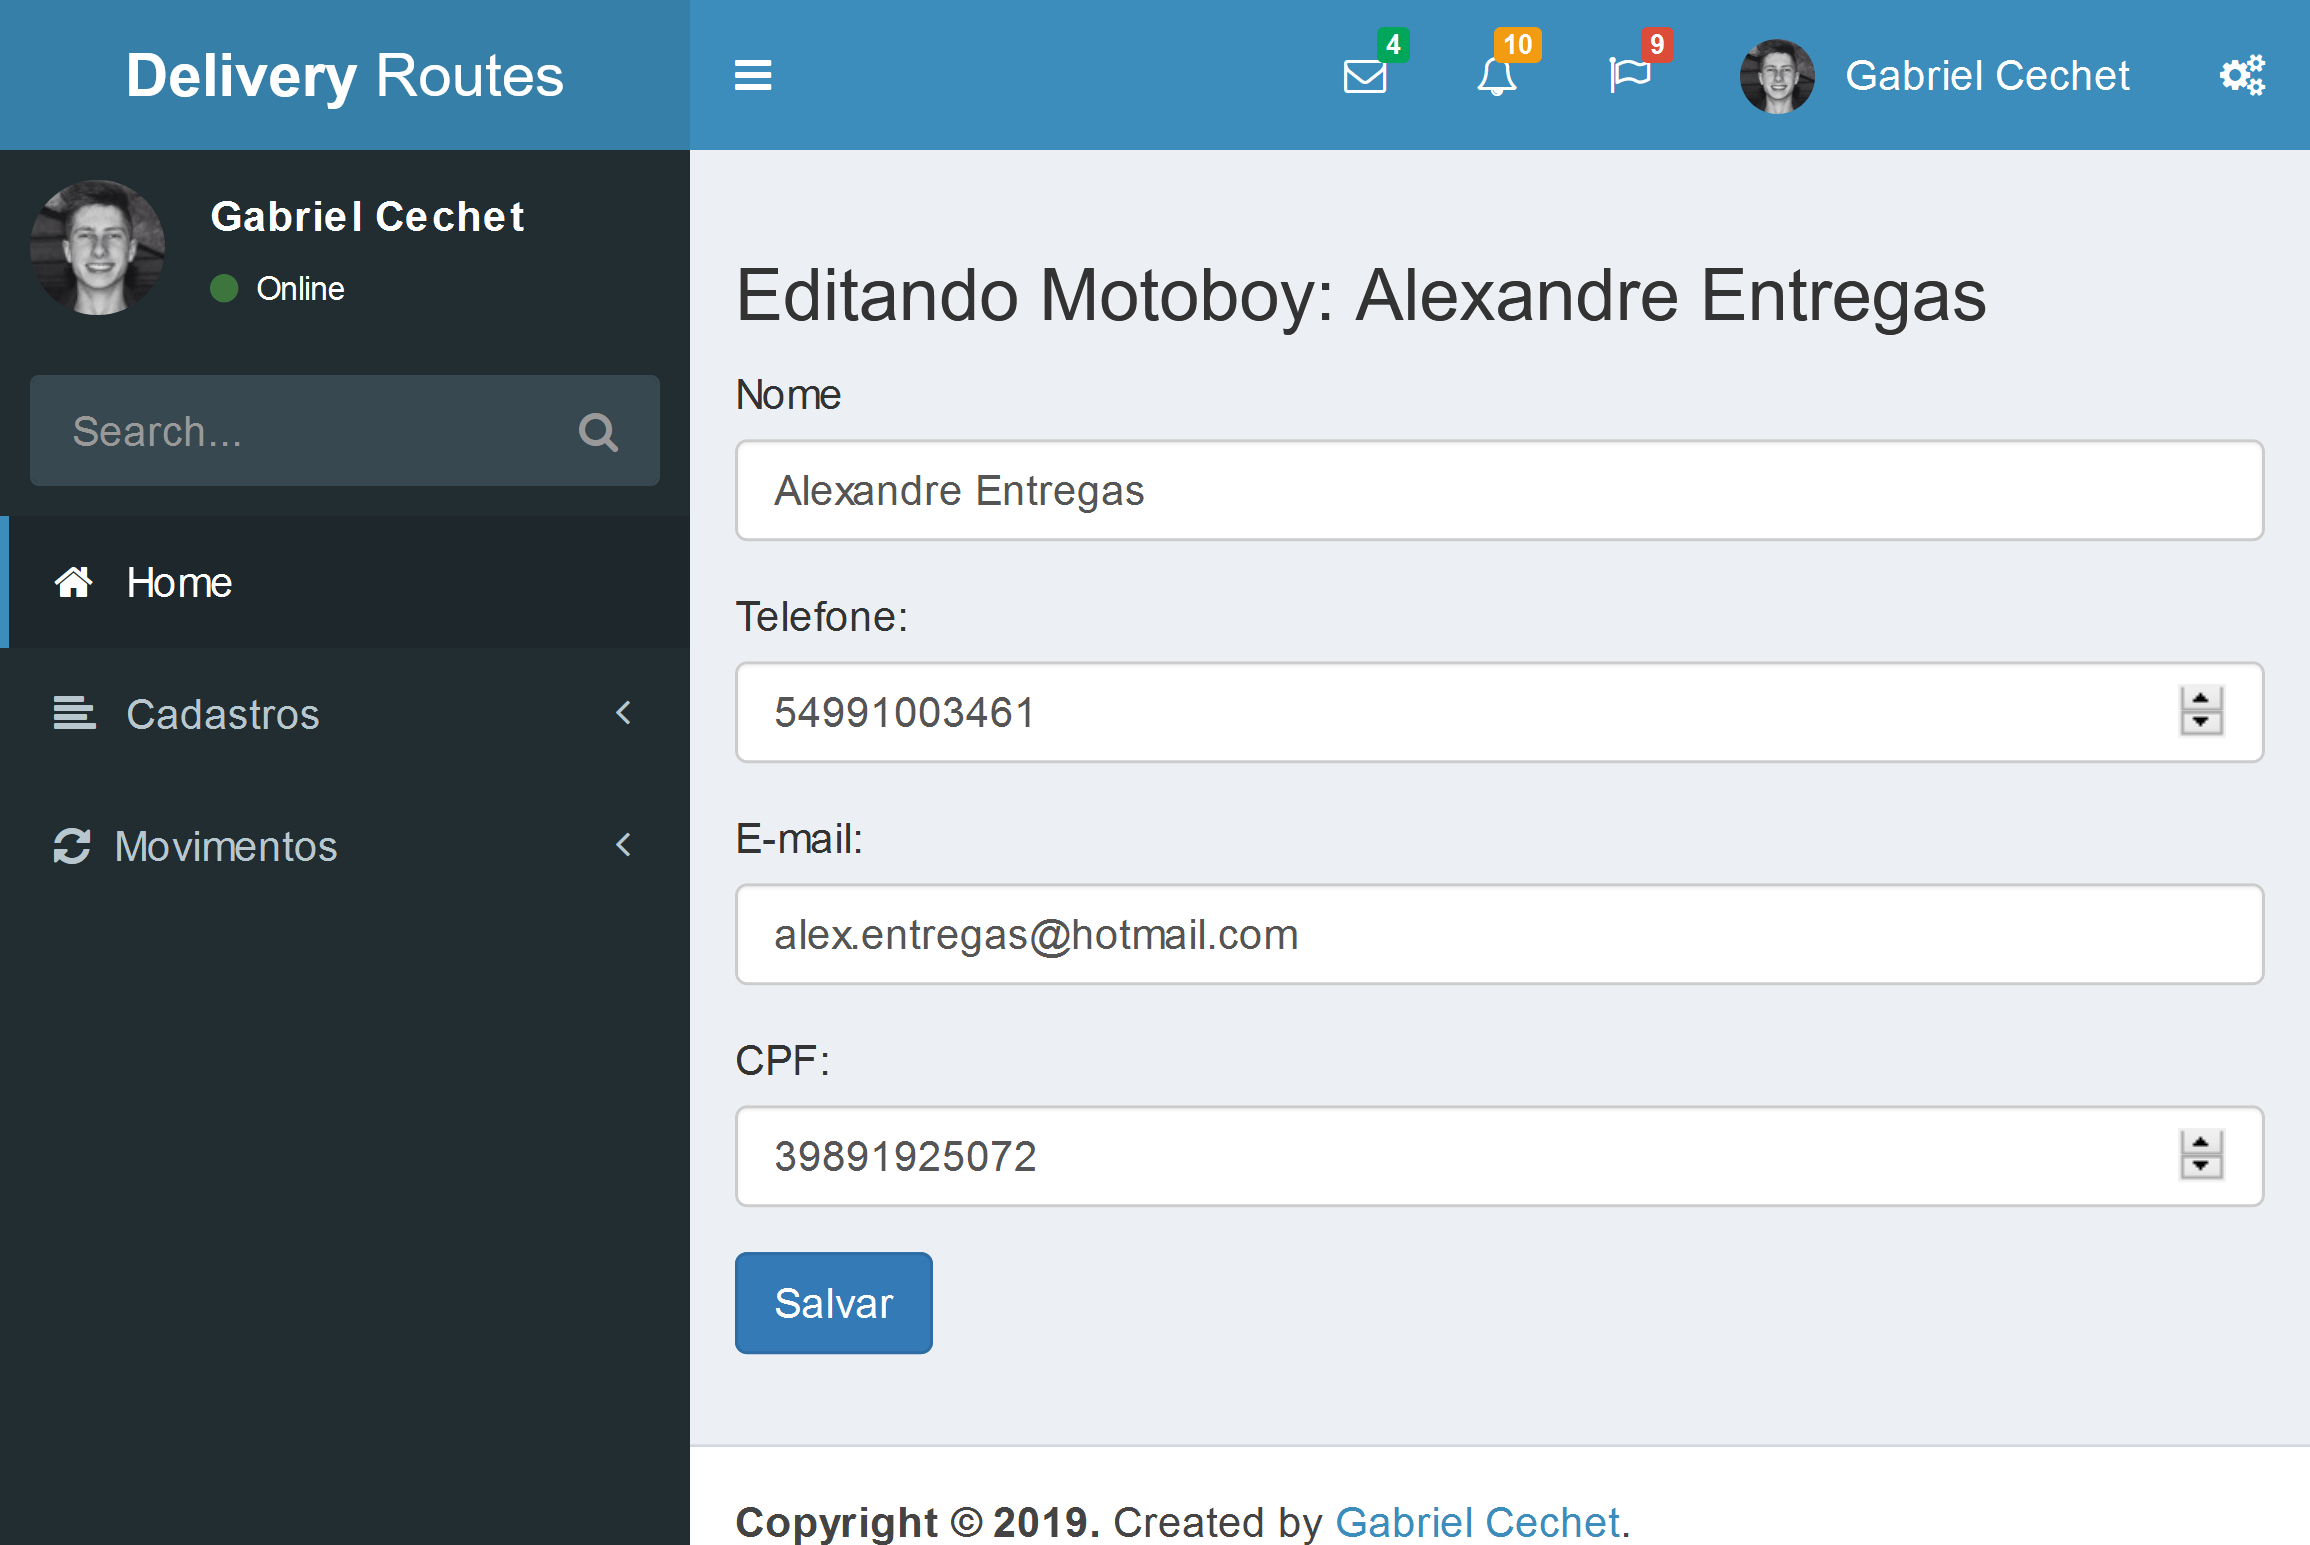
\includegraphics[width=1.0\textwidth]{./dados/figuras/fig19}
    \fonte{Autor}
    \label{fig:drEdicaoMotoby}
\end{figure}

\newpage
Igualmente à tela de motoboys, a tela de pagamentos possui uma listagem, dessa vez com o identificador e descrição dos registros cadastrados na base de dados, essa visualizada na \autoref{fig:drListaPagamentos}. 

A edição do registro é apresentada na \autoref{fig:drEdicaoPagamento}.

\begin{figure}[H]
    \centering
    \caption{Delivery Routes - Lista de pagamentos}
    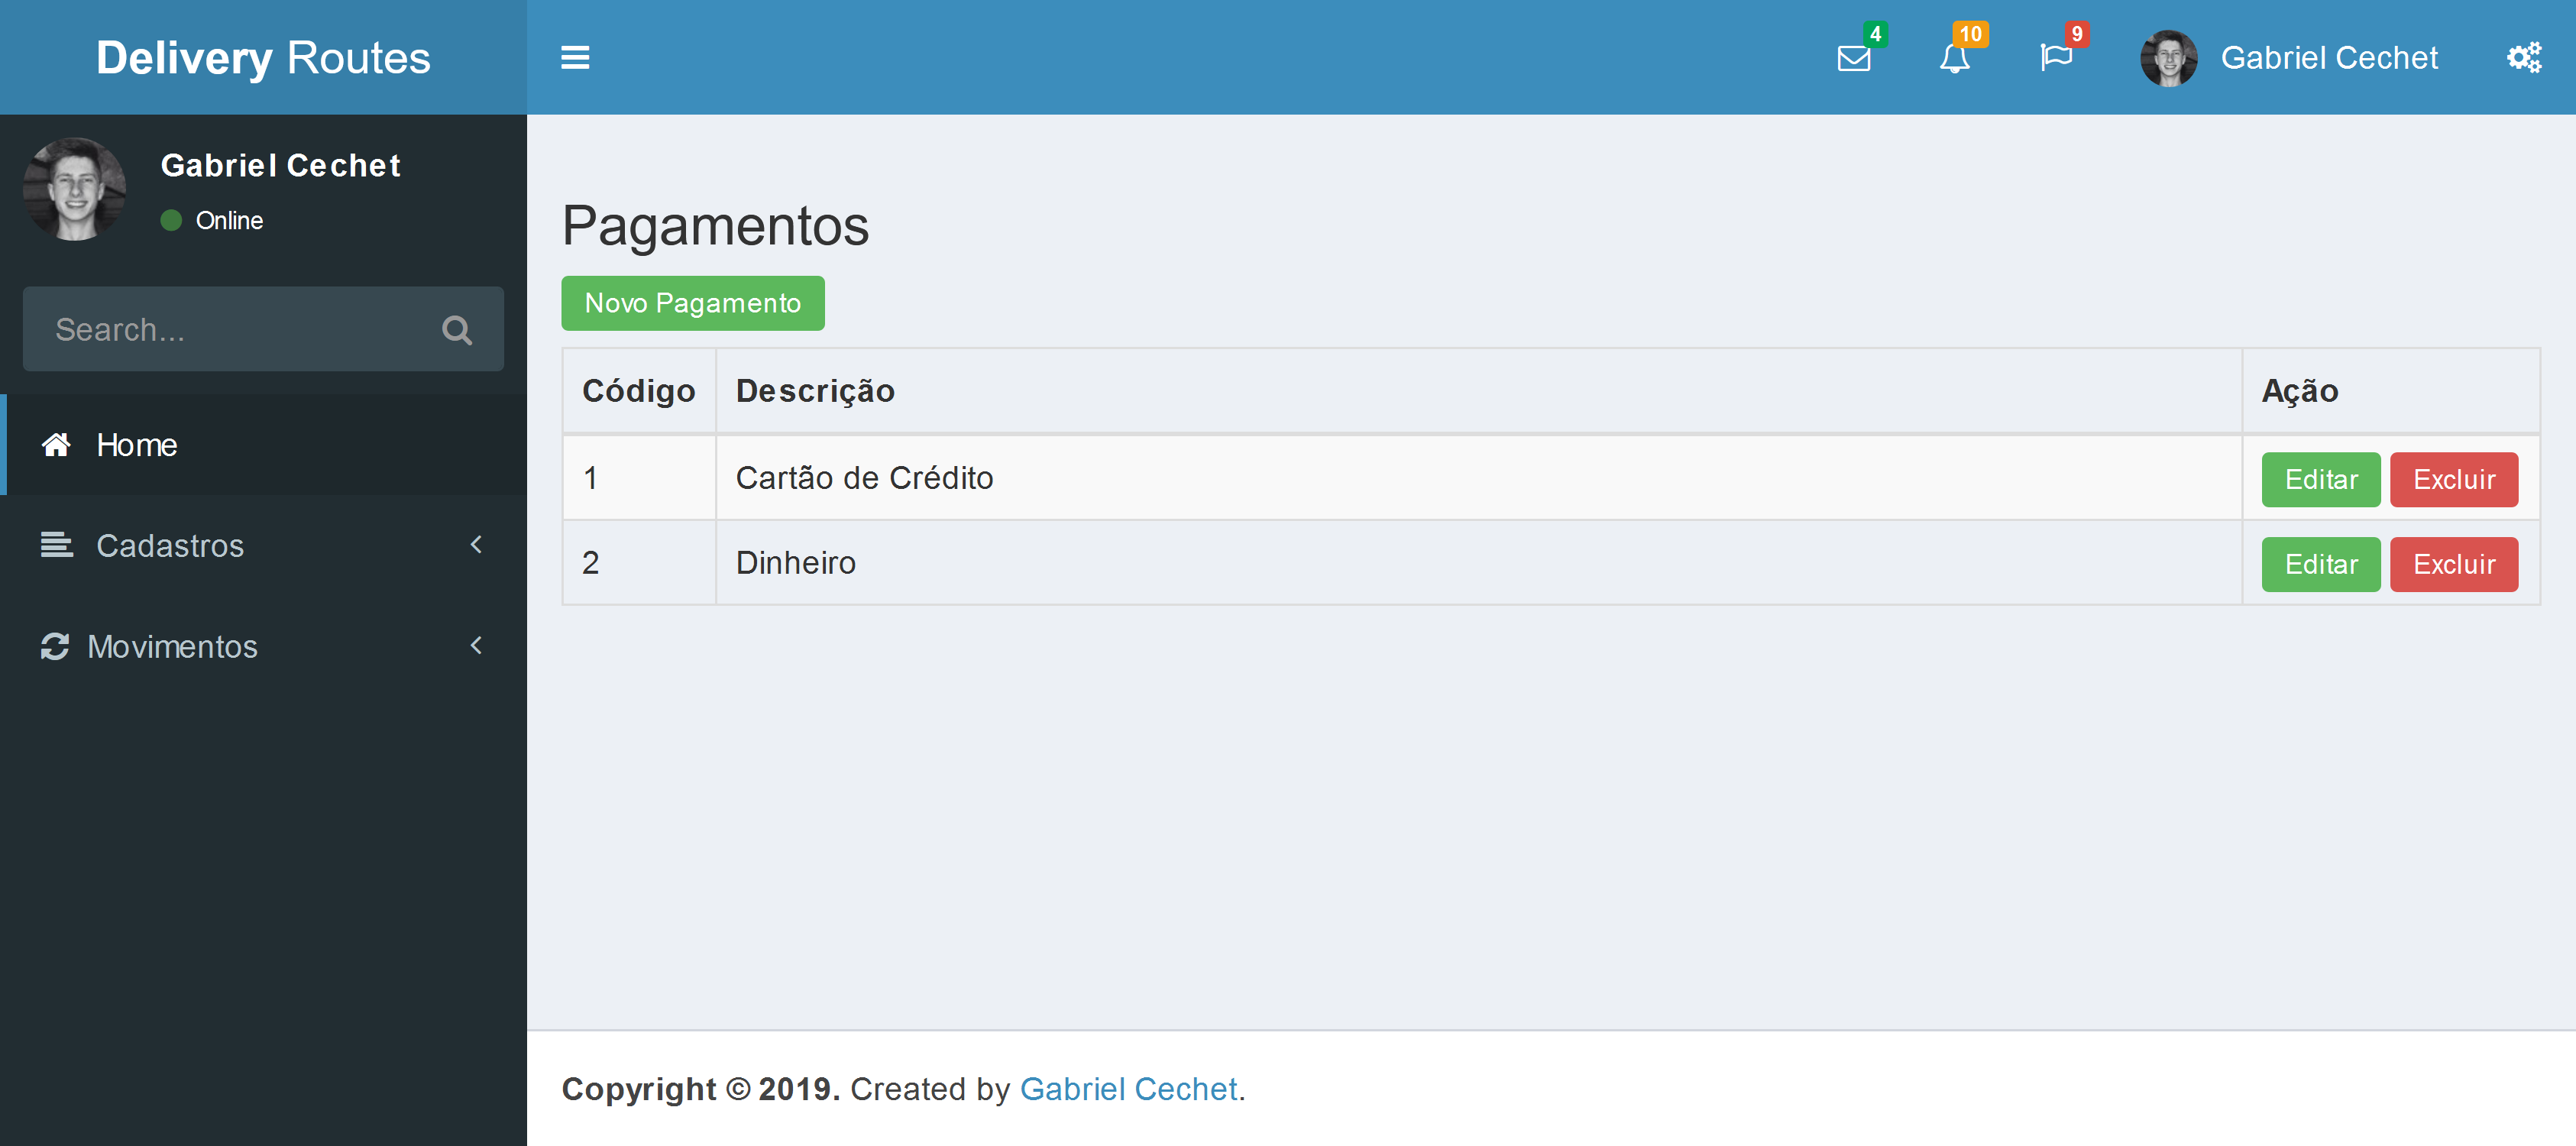
\includegraphics[width=1.0\textwidth]{./dados/figuras/fig20}
    \fonte{Autor}
    \label{fig:drListaPagamentos}
\end{figure}

\begin{figure}[H]
    \centering
    \caption{Delivery Routes - Edição do pagamento}
    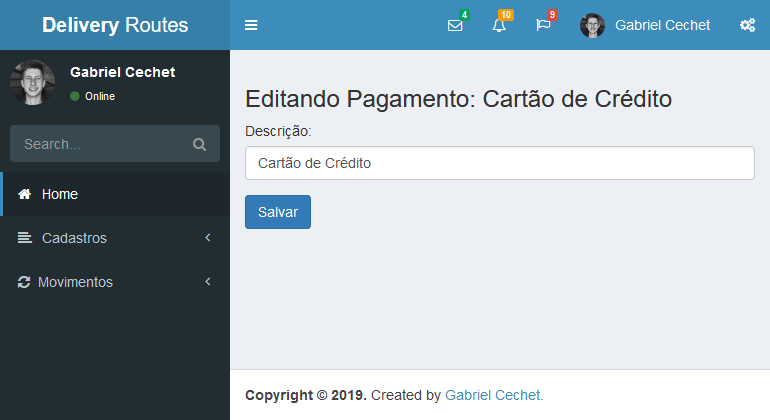
\includegraphics[width=1.0\textwidth]{./dados/figuras/fig21}
    \fonte{Autor}
    \label{fig:drEdicaoPagamento}
\end{figure}

\newpage
Ao selecionar a opção de menu “Entregas” (\autoref{fig:drListaEntregas}) é possível visualizar todo o histórico de entregas já realizadas na aplicação. Nela estão presentes informações como o identificador, motoboy, status e os pedidos que compõem cada entrega. Botões para visualização, impressão da comanda, finalização (altera o \textit{status} da entrega para \textit{CONCLUDED}) e cancelamento (altera o status da entrega para \textit{CANCELLED}) acompanham cada registro.

 \begin{figure}[H]
    \centering
    \caption{Delivery Routes - Lista de entregas}
    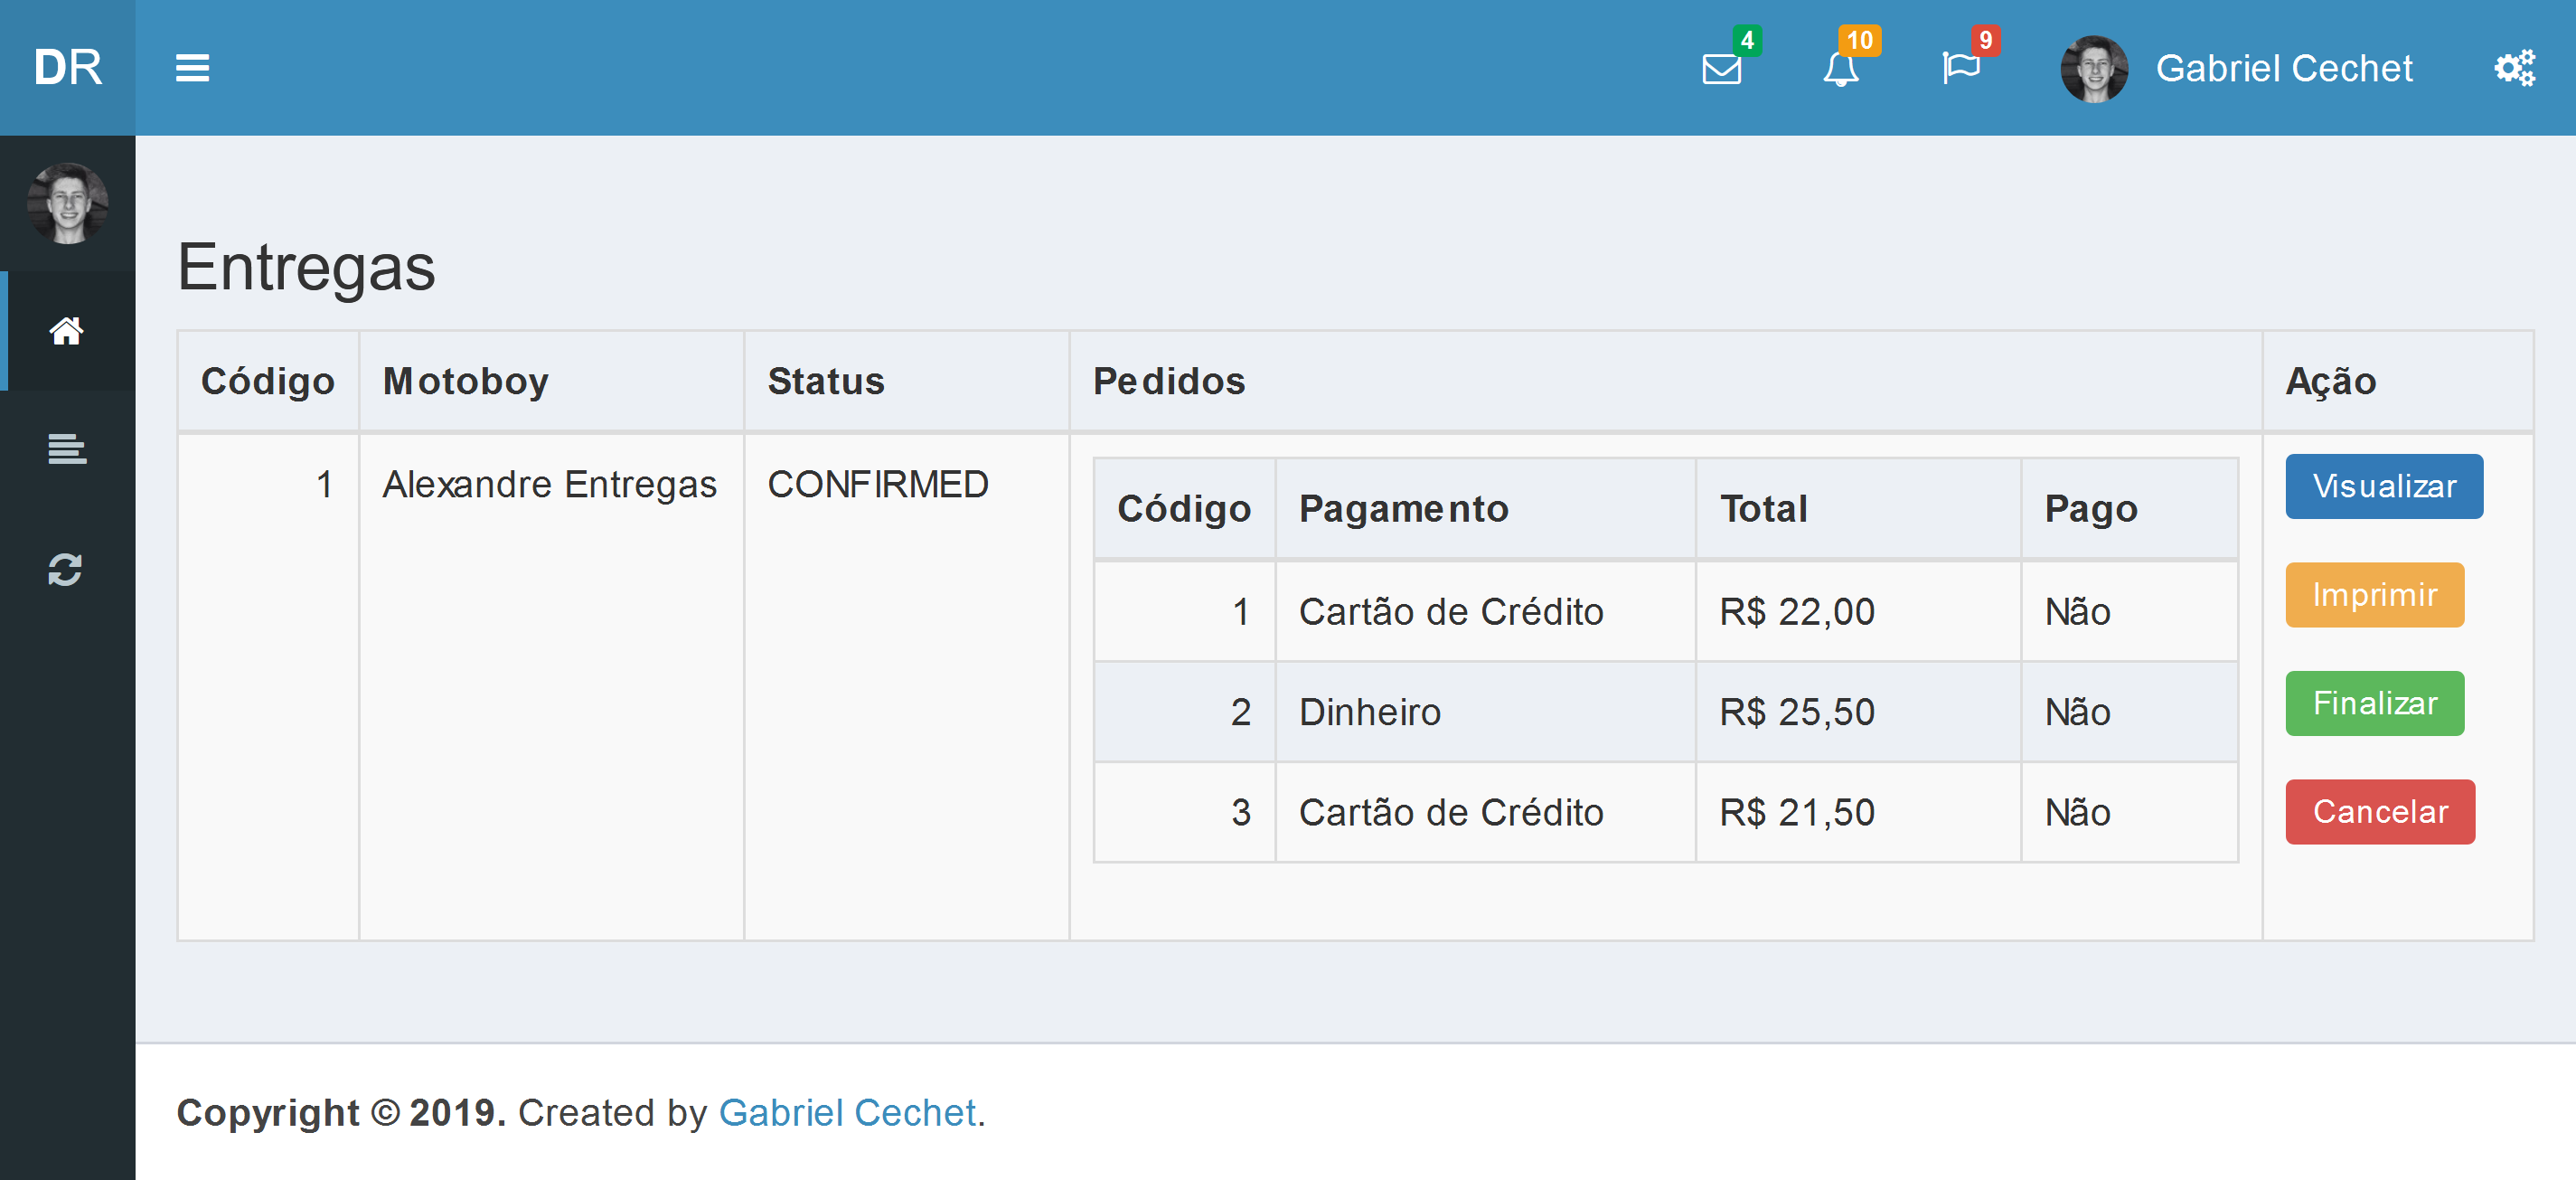
\includegraphics[width=1.0\textwidth]{./dados/figuras/fig26}
    \fonte{Autor}
    \label{fig:drListaEntregas}
\end{figure}

 \begin{figure}[H]
    \centering
    \caption{Delivery Routes - Lista de pedidos em aberto}
    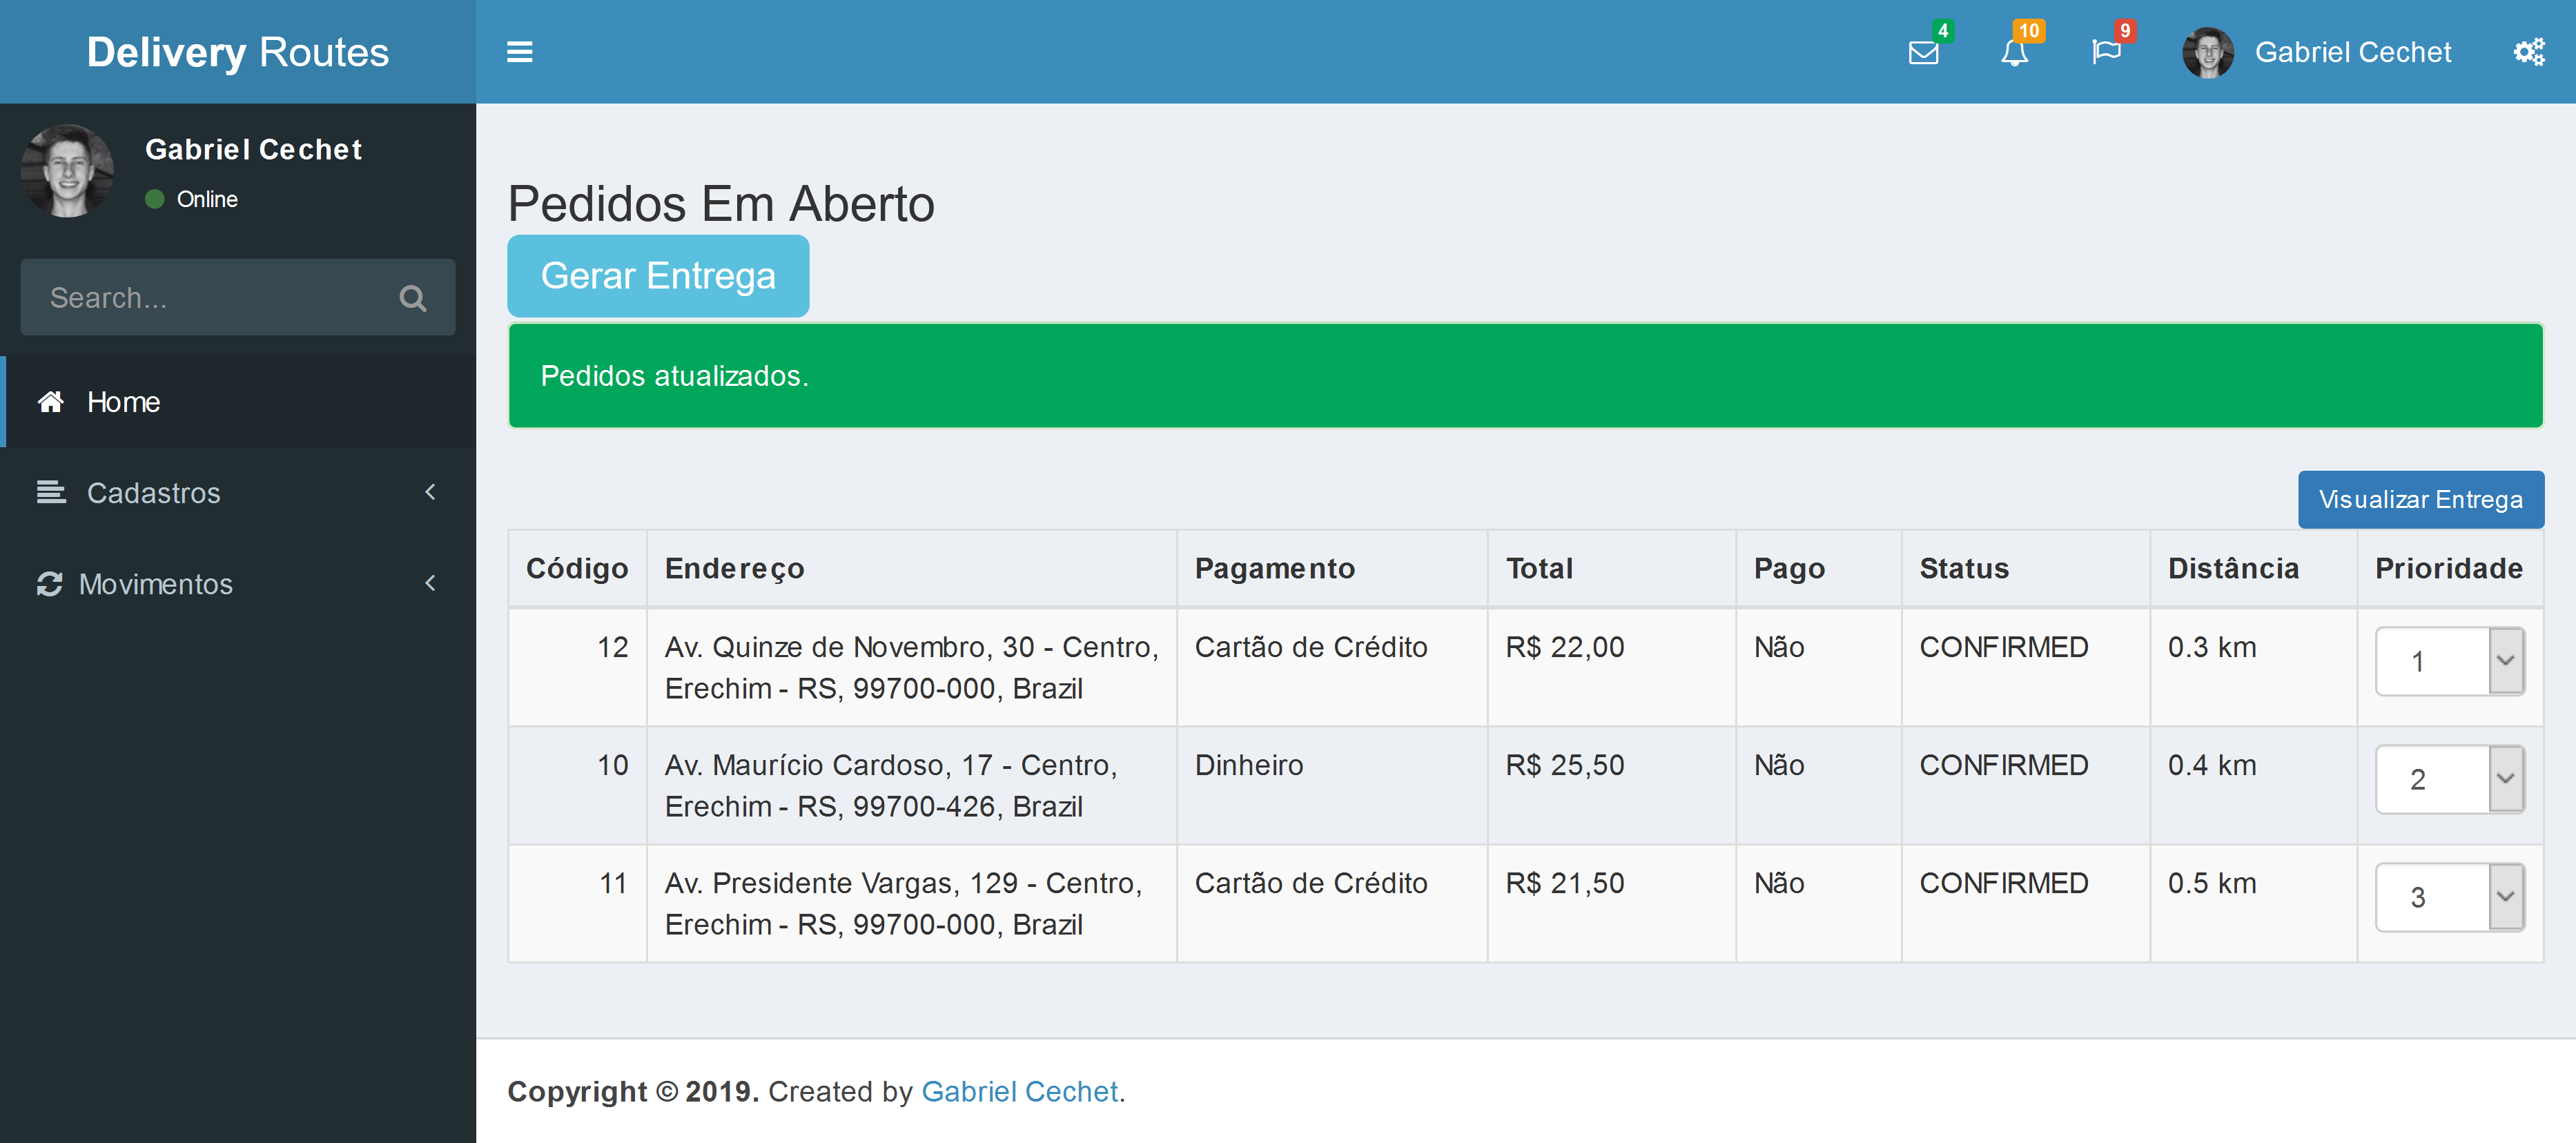
\includegraphics[width=1.0\textwidth]{./dados/figuras/fig29}
    \fonte{Autor}
    \label{fig:drListaPedidos}
\end{figure}

\newpage
Na \autoref{fig:drListaPedidos} é apresentada a tela de “Pedidos Em Aberto”, onde os dados são apresentados quando, via requisição \textit{GET} na rota \textit{“/orders/opened”} na API do software principal do estabelecimento, executada pela rota: \textit{/orders/index}. Como resposta o servidor informa um objeto JSON com a lista dos pedidos com status \textit{PLACED}. No \autoref{alg:orderIndex} é apresentada a função que integra os pedidos no Delivery Routes.

\begin{lstlisting}[caption={Delivery Routes - Função integradora de pedidos}, style=htmlcssjs, label=alg:orderIndex]
public function index() {
    $req = Request();
    $data = json_decode(file_get_contents('http://127.0.0.1:8000/orders/opened'));
    foreach ($data as $key => $item) {
            Order::create([
                    'id' => $item['id'],
                    'latitude' => $item['latitude'],
                    'longitude' => $item['longitude'],
                    'payment_id' => $item['payment_id'],
                    'totalPrice' => $item['totalPrice'],
                    'status' => 'PLACED']);
        $req->session()->flash('mensagem-sucesso', 'Pedidos atualizados.');
    }

    $this->changePriority();
    $orders = Order::all()->where('status', '=', 'CONFIRMED')->sortBy('priority');
    return view('orders.index', ['orders'=> $orders]);
}
\end{lstlisting}

Essa função executa, também, um método denominado \textit{changePriority()}, que por meio das APIs Distance Matrix e Geocoder do Google Maps, preenchem os campos \textit{distance} e \textit{formatted\_address} dos pedidos (\autoref{alg:changePriority}). Além disso, é feita a alteração do status dos pedidos integrados para \textit{CONFIRMED}.

A partir do campo \textit{distance}, preenchido anteriormente, é agregada a prioridade sugerida pela aplicação. A regra aplicada nessa etapa consiste em analisar qual o pedido se encontra mais próximo à posição do usuário no momento da requisição à Distance Matrix API.

Com todos os dados preenchidos (endereço, distância e prioridade), é possível analisar e gerenciar as informações sugeridas para cada pedido.

\newpage
\begin{lstlisting}[caption={Delivery Routes - Função de troca de prioridade dos pedidos}, style=htmlcssjs, label=alg:changePriority]
 private function changePriority() {
    $orders = Order::all()->where('status', '=', 'PLACED');
    foreach ($orders as $item) {
        $coordinates = GoogleMaps::geocodeAddress($item->latitude, $item->longitude);
        $distance = GoogleMaps::distanceMatrix($item->latitude, $item->longitude);
        $item->update(['formatted_address' => $coordinates['formatted_address'], 'status' => 'CONFIRMED', 'distance' => $distance['distance']]);
    }

    $orders = Order::all()->where('status', '=', 'CONFIRMED')->sortBy('distance');
    $priority = 1;
    foreach ($orders as $item) {
        $item->update(['priority' => $priority]);
        $priority++;
    }
}
\end{lstlisting}